%http://www2.informatik.uni-freiburg.de/~frank/ENG/latex-course/latex-course-3/latex-course-3_en.html
\documentclass{beamer}
%beamer options
\usetheme{Rochester}
\usecolortheme{beaver}

%packages
\usepackage[T1]{fontenc}
\usepackage[utf8]{inputenc}
\usepackage[italian]{babel}
\usepackage{graphicx}
\usepackage{hyperref}
\usepackage{url}

%macro
%\AtBeginSection{\frame{\sectionpage}}
%\renewcommand{\sectionname}{Sezione}

\begin{document}
\title{Distribuzione di dati aperti e riutilizzo dell'informazione}  
\author{Stefano Sabatini}
\date{24/07/14} 

\begin{frame}
\titlepage
\end{frame}

\begin{frame}
\frametitle{Indice}
\begin{itemize}
\item Open Source ed Open Knowledge
\item Linked Open Data
\item Valutazione dei dati
\item Distribuzione e pacchettizzazione dei dati
\item Open Data nella legislazione italiana
\item Conclusioni
\item Scraping autovelox
\item Genoa Port Stats
\item Licenze
\end{itemize}
\end{frame}

\begin{frame}
\frametitle{Indice}
\begin{itemize}
\item Open Source ed Open Knowledge
\item \textbf{Linked Open Data}
\item \textbf{Valutazione dei dati}
\item Distribuzione e pacchettizzazione dei dati
\item Open Data nella legislazione italiana
\item Conclusioni
\item \textbf{Scraping autovelox}
\item \textbf{Genoa Port Stats}
\item Licenze
\end{itemize}
\end{frame}

\begin{frame}
\frametitle{Open Data} 
\begin{itemize}
\item Il discorso sulle libertà informatiche si è progressivamente spostato alla disponibilità di informazione in formato aperto
\item Un dato si dice aperto se rispetta diversi criteri tra i quali ad esempio:
\begin{itemize}
\item deve avere formato aperto ed essere processabile in automatico
\item essere distribuibile e riutilizzabile anche commercialmente
\item esser completo (non aggregato) ed accessibile
\end{itemize} 
\end{itemize} 
\end{frame}

\begin{frame}
\frametitle{Linked Data} 
\begin{itemize}
\item Tim Berners-Lee ipotizza il Web Semantico, nel quale anche i dati sono "navigabili" (\emph{linked data})
\item I dati non solo devono essere liberamente accessibili e processabili da computer ma anche collegati fra di loro (\emph{linked open data})
\item Scala di valutazione dei dati che ha nel livello più alto i linked data
\end{itemize} 
\end{frame}

\begin{frame}
\frametitle{Modelli di valutazione} 
Esistono altri modelli che considerano aspetti diversi:
\begin{itemize}
\item \textbf{Open Data Engagement}: misura il grado di partecipazione di chi rilascia i dati.
\item \textbf{ODI Certificates}: misura il potenziale economico della corretta pubblicazione di un dato
\item \textbf{Open Data Census}: controlla la presenza e la qualità di un insieme di dati "di valore" a livello nazionale e locale
\item \textbf{Open Government}: linee guida a cui si devono uniformare dati prodotti dagli enti pubblici
\end{itemize} 
\end{frame}
%a voce

\begin{frame}
\frametitle{Casi di studio} 
\begin{itemize}
\item In generale esistono uno o più provider di dati (per esempio la PA) ed un insieme di utilizzatori degli stessi
\item Nei casi di studio sono partito da ''closed data'', trasformandoli in open data
\item In seguito ho sviluppato applicazioni sulla base di questi dati

\begin{itemize}
\item Autovelox
\item GenoaPortStats
\end{itemize}

\end{itemize}
\end{frame}

\begin{frame}
\frametitle{Autovelox - Dati di partenza} 
\begin{figure}
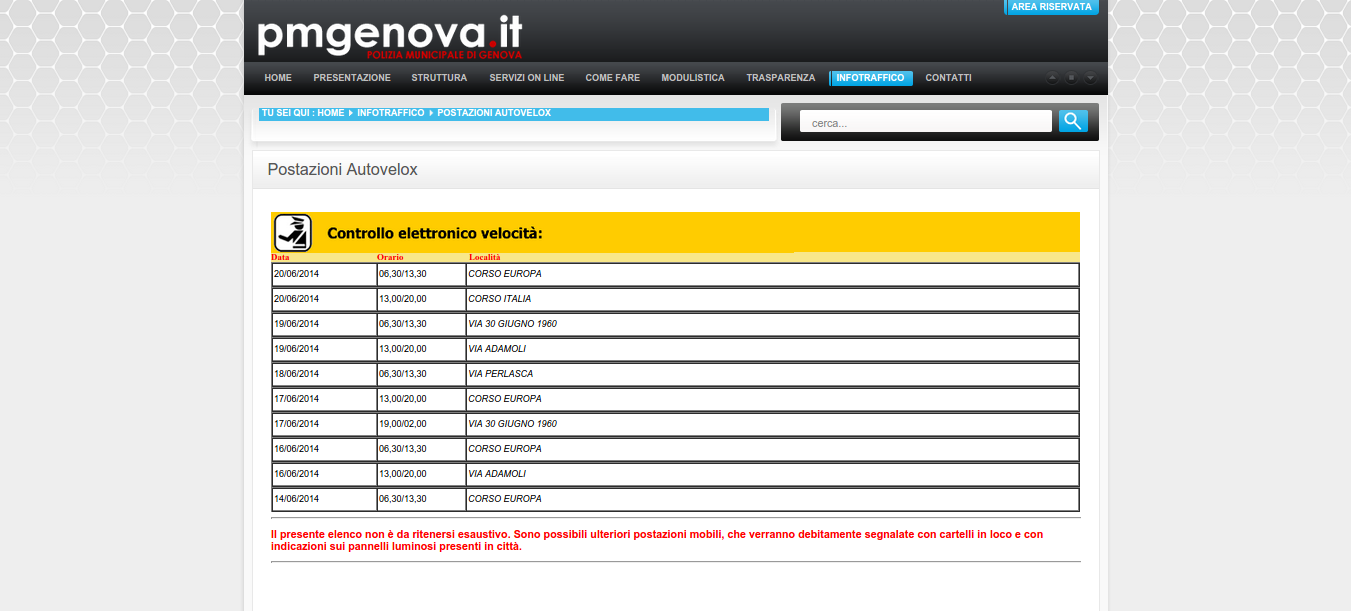
\includegraphics[width=\textwidth]{../img/Morph_PM_page.png} 
\end{figure}
Tabella HTML pubblicata sul sito della Polizia Municipale
\end{frame}

\begin{frame}
\frametitle{Autovelox - Scraping} 
\begin{figure}
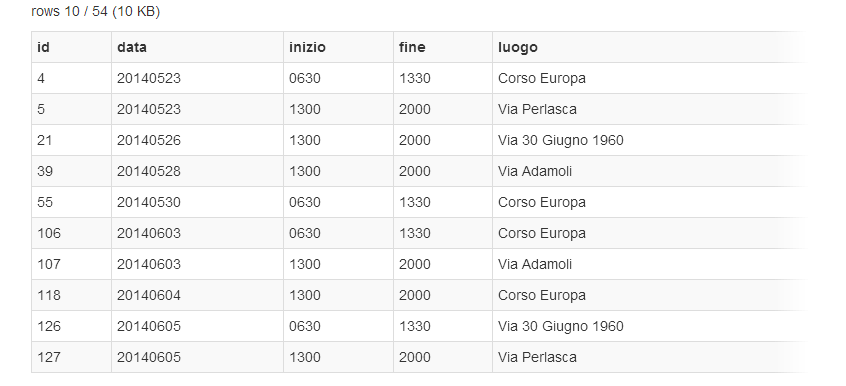
\includegraphics[width=\textwidth]{../img/Morph_home_2_cut.png} 
\end{figure}
Tramite estrazione automatica (lettura del DOM via PHP), viene aggiornato un database, liberamente utilizzabile tramite API all'url \href{https://morph.io/sabas/pmgenova_autovelox}{morph.io/sabas/pmgenova\_autovelox}.
\end{frame}

\begin{frame}
\frametitle{Autovelox - Applicazione dimostrativa} 
\begin{columns}
\begin{column}{6cm}
\begin{itemize}
\item Web-app scritta con framework AppJS
\item Sfrutta le API con PHP e JSONP
\item JSONP $\rightarrow$ \href{http://map.genova.it/autovelox/}{map.genova.it/autovelox}
\end{itemize}
\end{column}
\begin{column}{4cm}
\begin{figure}
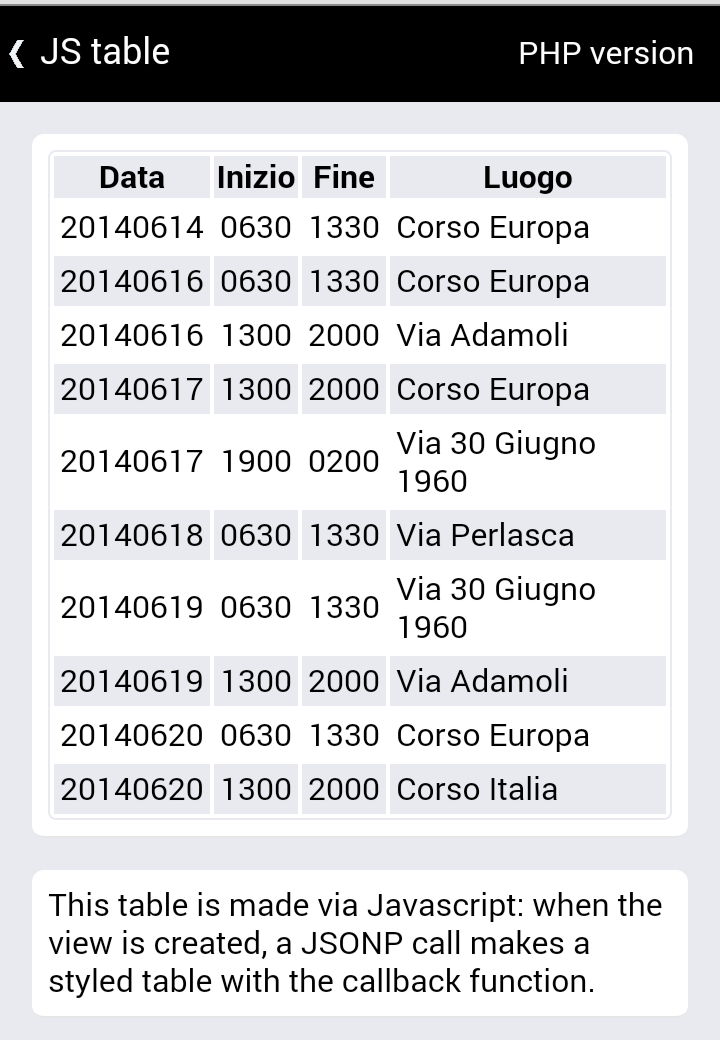
\includegraphics[width=\textwidth]{../img/autovelox_m3.png} 
\end{figure}
\end{column}
\end{columns}
\end{frame}

\begin{frame}
\frametitle{GenoaPortStats - Dati di partenza} 
\begin{figure}

\includegraphics[width=\textwidth]{../img/autorita.png} 
\end{figure}
\begin{itemize}
\item L'Autorità Portuale di Genova pubblica statistiche sul traffico
\item Queste sono in PDF, non riutilizzabili
\item Si possono "liberare" ed usare per visualizzazioni
\end{itemize}
\end{frame}

\begin{frame}
\frametitle{GenoaPortStats - Processo di sviluppo} 
I PDF sono stati:
\begin{itemize}
\item trasformati con Tabula e Calc in file TSV,
\item processati con script PHP (geocoding, normalizzazione),
\item visualizzati con diverse librerie (es. Leaflet).
\end{itemize}
I file ottenuti sono stati anche resi scaricabili in formati \emph{machine readable}.
Le licenze di utilizzo sono state esplicitate in conformità con i criteri di apertura dei dati.
\end{frame}

\begin{frame}
\frametitle{GenoaPortStats - Sito web}
\href{http://stefanosabatini.eu/GenoaPortStats/}{http://stefanosabatini.eu/GenoaPortStats/}
\begin{figure}
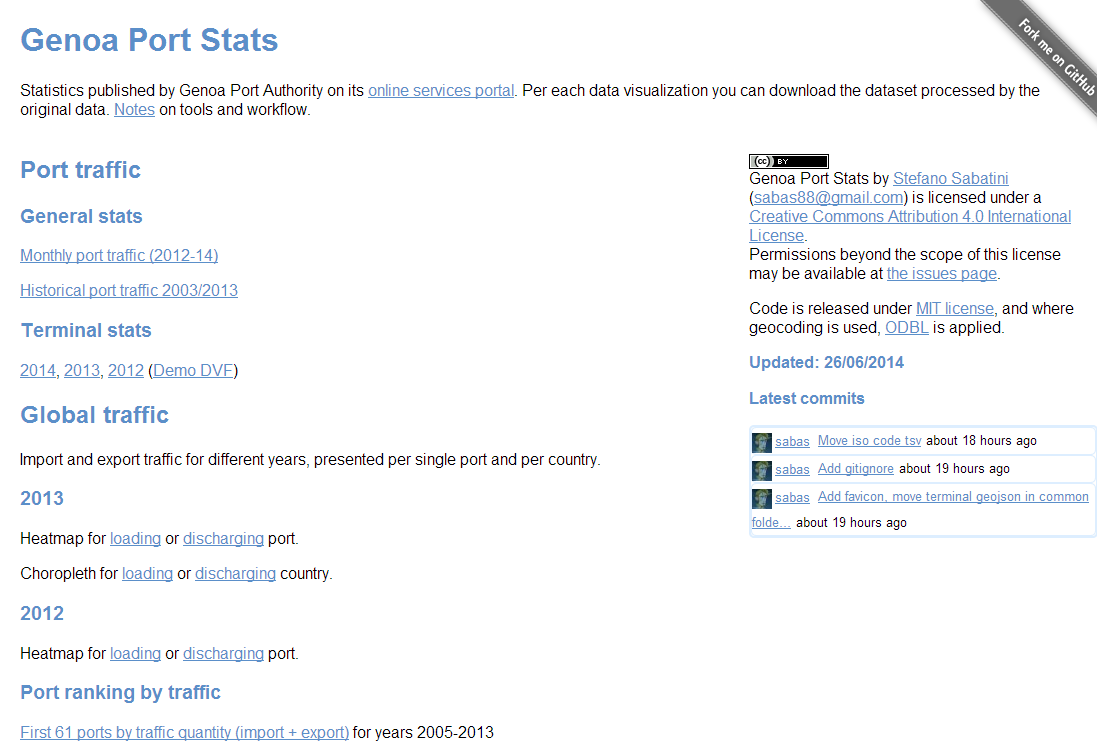
\includegraphics[width=\textwidth]{../img/portstats_home.png} 
\end{figure}
\end{frame}

\begin{frame}
\frametitle{GenoaPortStats - Heatmap} 
\begin{figure}
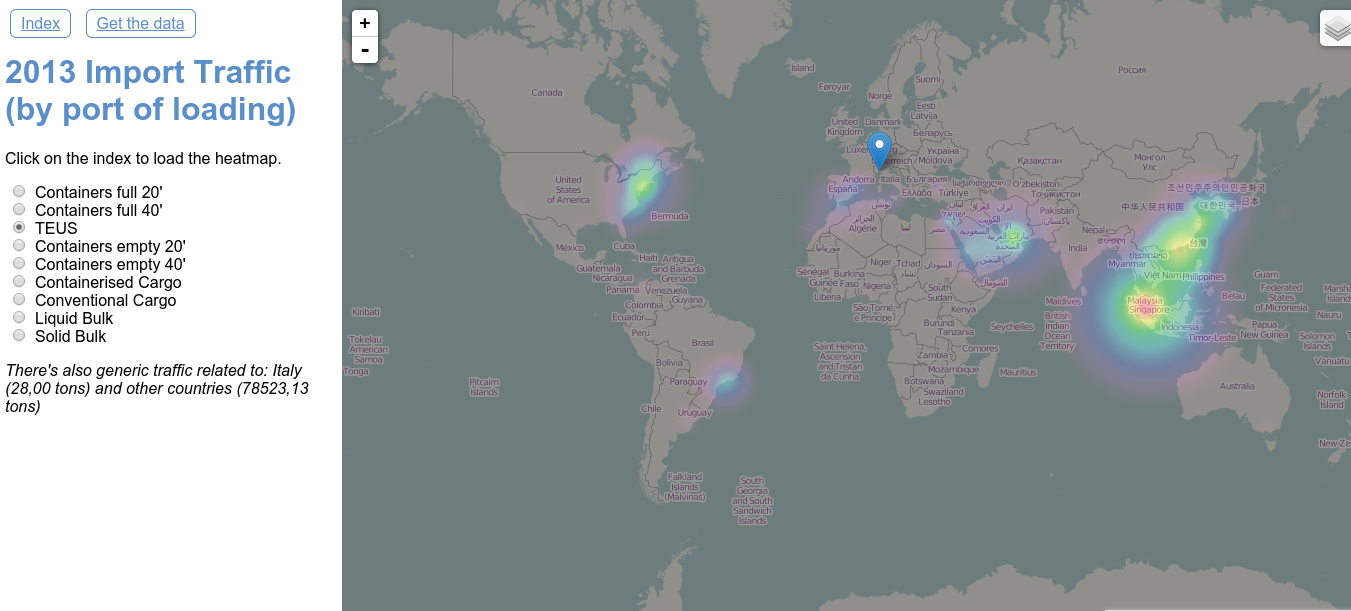
\includegraphics[width=\textwidth]{../img/portstats_loadingtraffic.png} 
\end{figure}
\end{frame}

\begin{frame}
\frametitle{GenoaPortStats - Cartogramma} 
\begin{figure}
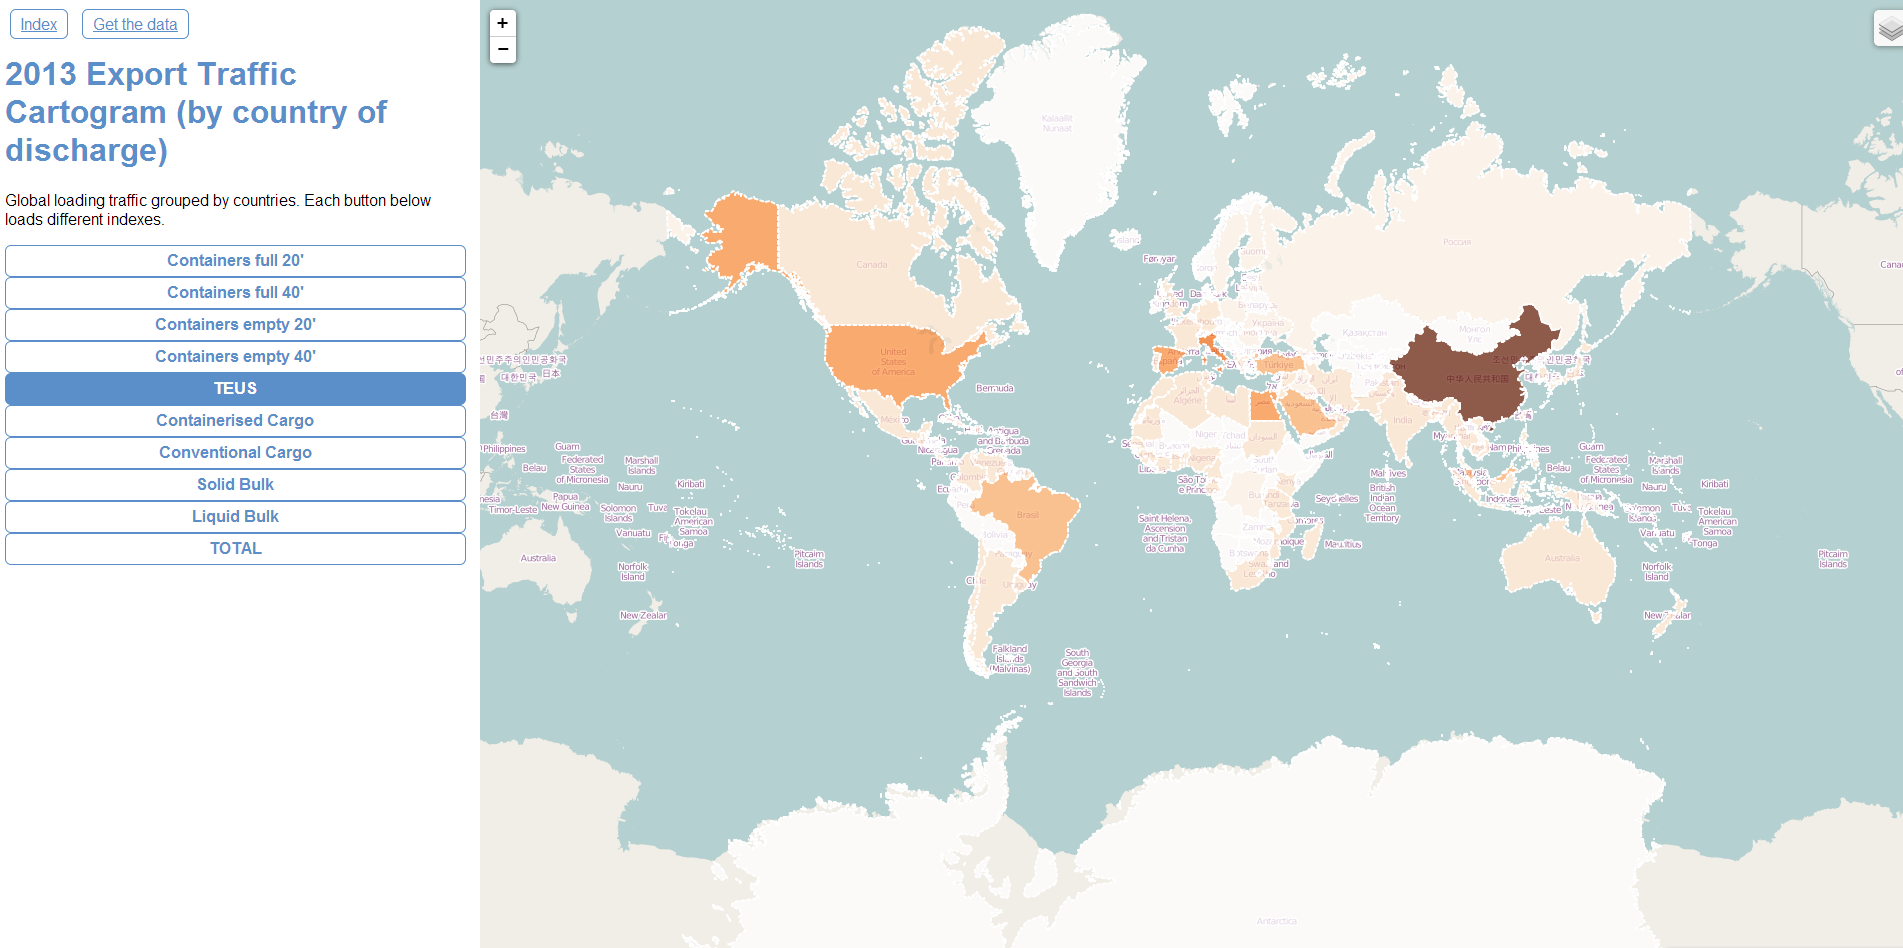
\includegraphics[width=\textwidth]{../img/portstats_cartogram.png} 
\end{figure}
\end{frame}

\begin{frame}
\frametitle{GenoaPortStats - Choropleth} 
\begin{figure}
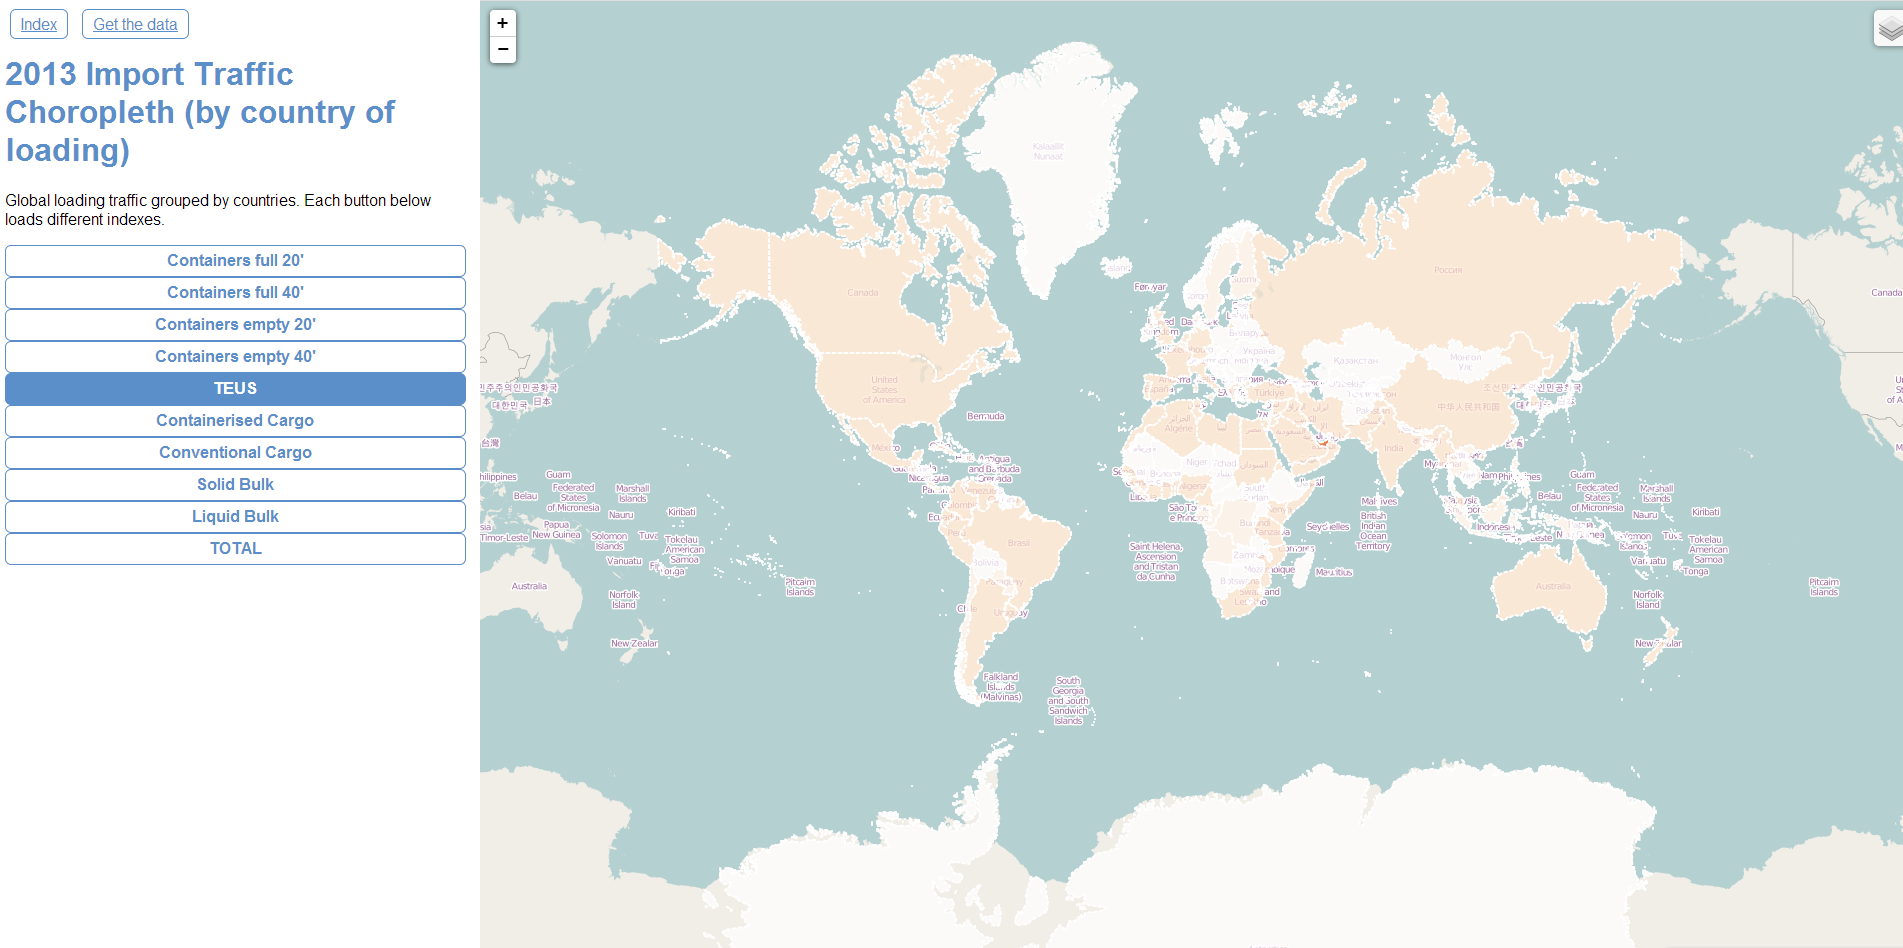
\includegraphics[width=\textwidth]{../img/portstats_choropleth.png} 
\end{figure}
\end{frame}

\begin{frame}
\frametitle{GenoaPortStats - Quota porti collegati} 
\begin{figure}
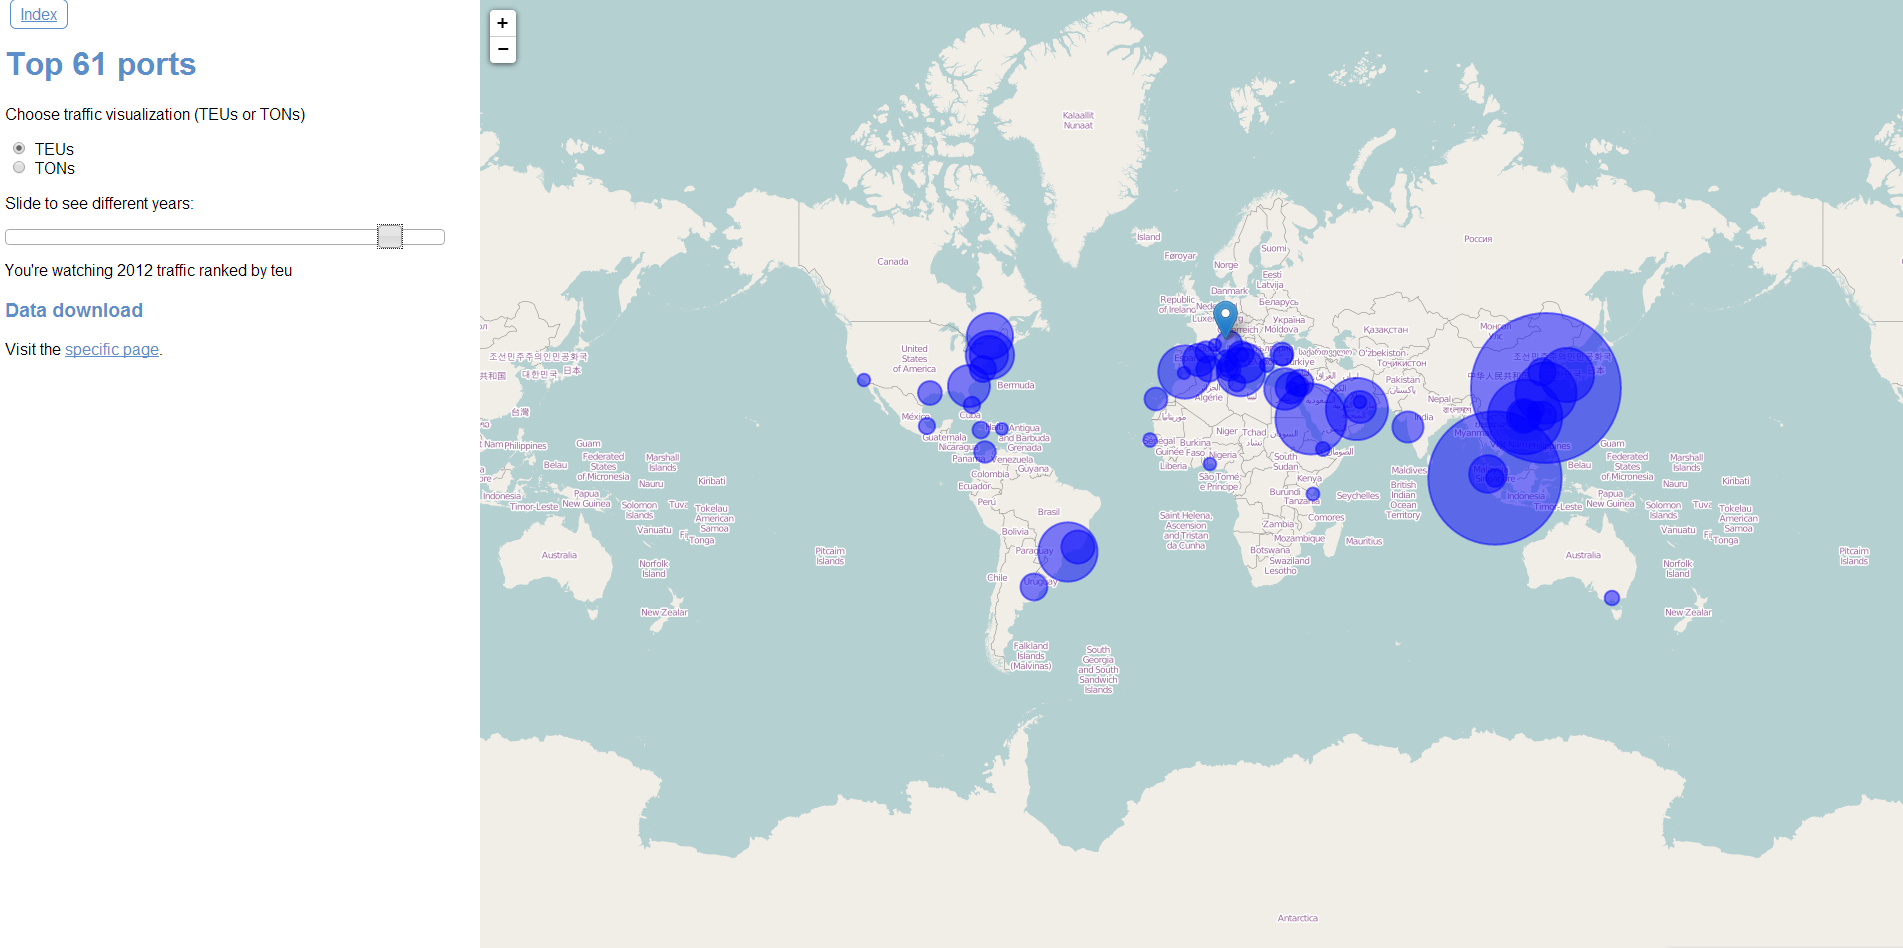
\includegraphics[width=\textwidth]{../img/genoaportstats_top61_interface2012.png} 
\end{figure}
\end{frame}

\begin{frame}
\frametitle{GenoaPortStats - Traffico storico del porto} 
\begin{figure}
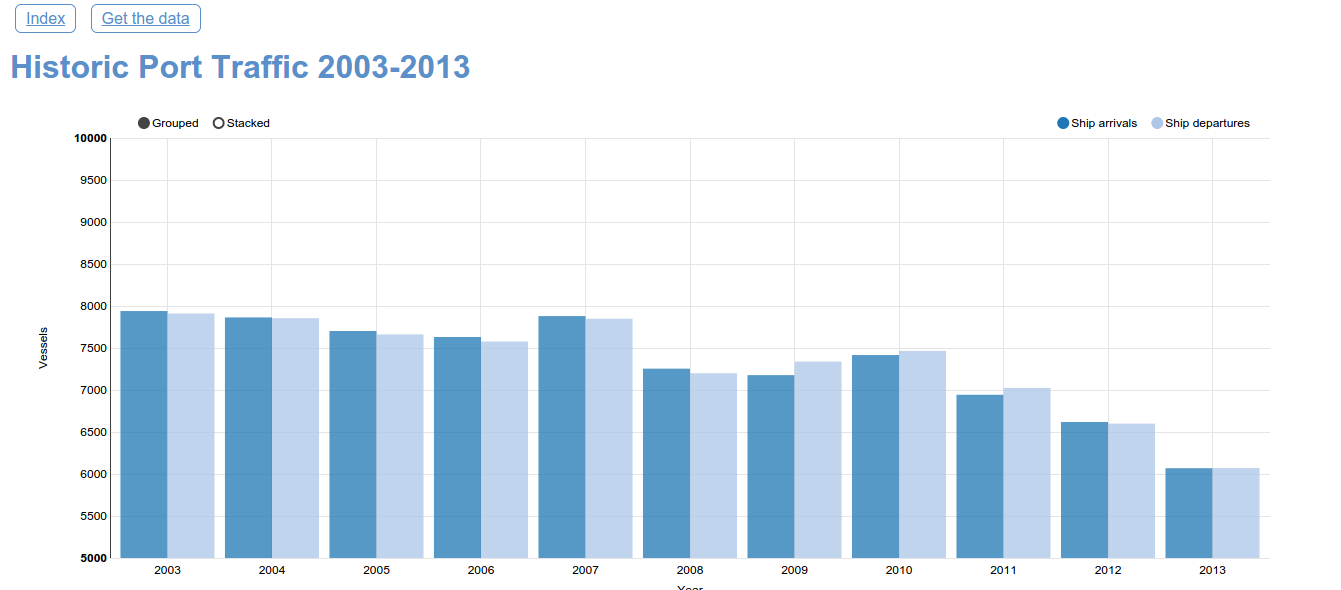
\includegraphics[width=\textwidth]{../img/portstats_historic.png} 
\end{figure}
\end{frame}

\begin{frame}
\frametitle{GenoaPortStats - Traffico mensile dei terminal} 
\begin{figure}
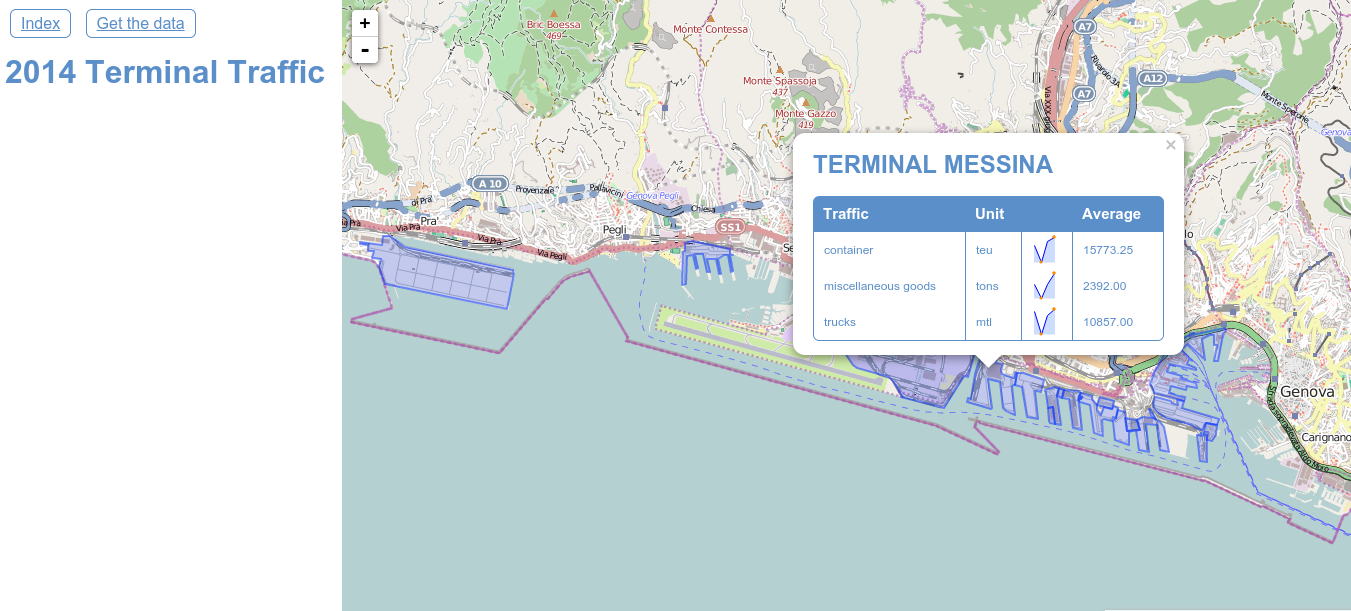
\includegraphics[width=\textwidth]{../img/portstats_terminal.png} 
\end{figure}
\end{frame}

\begin{frame}[plain,c]
\begin{center}
\Huge Grazie
\end{center}
\end{frame}
\end{document}
